\documentclass[msc,lith,english]{liuthesis}
%DIF LATEXDIFF DIFFERENCE FILE
%DIF DEL b.tex   Mon Nov 28 12:28:56 2022
%DIF ADD a.tex   Mon Nov 28 12:24:20 2022

%%%%%%%%%%%%%%%%%%%%%%%%%%%%%%%%%%%%%%%%%%%%%%%%%
% Imports
%%%%%%%%%%%%%%%%%%%%%%%%%%%%%%%%%%%%%%%%%%%%%%%%%
%\usepackage[english]{babel}
\usepackage[utf8]{inputenc}
%DIF 8c8
%DIF < \usepackage[backend=biber,sorting=none]{biblatex}
%DIF -------
\usepackage[backend=biber,sorting=none,hyperref]{biblatex} %DIF > 
%DIF -------
\usepackage{mathtools}
\usepackage{dsfont}
\usepackage{tikz}
%DIF 12c12-13
%DIF < \usetikzlibrary{topaths,calc}
%DIF -------
\usetikzlibrary{topaths,calc,tikzmark} %DIF > 
\usepackage{algorithm2e} %DIF > 
%DIF -------

%%%%%%%%%%%%%%%%%%%%%%%%%%%%%%%%%%%%%%%%%%%%%%%%%
% Settings
%%%%%%%%%%%%%%%%%%%%%%%%%%%%%%%%%%%%%%%%%%%%%%%%%
\department{Institutionen för datavetenskap}
\departmentenglish{Department of Computer and Information Science}
\departmentshort{IDA}

\supervisor{Peter Jonson}
\examiner{???}
\titleenglish{A Faster Algoritm for Solving the No-Rainbow Problem}
\subtitleenglish{100\% rainbow-free guarantee}
\titleswedish{En snabbare algoritm för No Rainbow problemet}
\thesissubject{Datavetenskap}

\publicationyear{2023}
\currentyearthesisnumber{001}
\dateofpublication{2023-01-20}

\addbibresource{thesis.bib}
%DIF 33a34-38
 %DIF > 
\newcommand\tikznode[3][]% %DIF > 
   {\tikz[remember picture, baseline=(#2.base)] %DIF > 
      \node[minimum size=0pt,inner sep=0pt,#1](#2){#3};% %DIF > 
   } %DIF > 
%DIF -------

\author{Edvard Thörnros}
%DIF PREAMBLE EXTENSION ADDED BY LATEXDIFF
%DIF UNDERLINE PREAMBLE %DIF PREAMBLE
\RequirePackage[normalem]{ulem} %DIF PREAMBLE
\RequirePackage{color}\definecolor{RED}{rgb}{1,0,0}\definecolor{BLUE}{rgb}{0,0,1} %DIF PREAMBLE
\providecommand{\DIFadd}[1]{{\protect\color{blue}\uwave{#1}}} %DIF PREAMBLE
\providecommand{\DIFdel}[1]{{\protect\color{red}\sout{#1}}}                      %DIF PREAMBLE
%DIF SAFE PREAMBLE %DIF PREAMBLE
\providecommand{\DIFaddbegin}{} %DIF PREAMBLE
\providecommand{\DIFaddend}{} %DIF PREAMBLE
\providecommand{\DIFdelbegin}{} %DIF PREAMBLE
\providecommand{\DIFdelend}{} %DIF PREAMBLE
\providecommand{\DIFmodbegin}{} %DIF PREAMBLE
\providecommand{\DIFmodend}{} %DIF PREAMBLE
%DIF FLOATSAFE PREAMBLE %DIF PREAMBLE
\providecommand{\DIFaddFL}[1]{\DIFadd{#1}} %DIF PREAMBLE
\providecommand{\DIFdelFL}[1]{\DIFdel{#1}} %DIF PREAMBLE
\providecommand{\DIFaddbeginFL}{} %DIF PREAMBLE
\providecommand{\DIFaddendFL}{} %DIF PREAMBLE
\providecommand{\DIFdelbeginFL}{} %DIF PREAMBLE
\providecommand{\DIFdelendFL}{} %DIF PREAMBLE
%DIF COLORLISTINGS PREAMBLE %DIF PREAMBLE
\RequirePackage{listings} %DIF PREAMBLE
\RequirePackage{color} %DIF PREAMBLE
\lstdefinelanguage{DIFcode}{ %DIF PREAMBLE
%DIF DIFCODE_UNDERLINE %DIF PREAMBLE
  moredelim=[il][\color{red}\sout]{\%DIF\ <\ }, %DIF PREAMBLE
  moredelim=[il][\color{blue}\uwave]{\%DIF\ >\ } %DIF PREAMBLE
} %DIF PREAMBLE
\lstdefinestyle{DIFverbatimstyle}{ %DIF PREAMBLE
	language=DIFcode, %DIF PREAMBLE
	basicstyle=\ttfamily, %DIF PREAMBLE
	columns=fullflexible, %DIF PREAMBLE
	keepspaces=true %DIF PREAMBLE
} %DIF PREAMBLE
\lstnewenvironment{DIFverbatim}{\lstset{style=DIFverbatimstyle}}{} %DIF PREAMBLE
\lstnewenvironment{DIFverbatim*}{\lstset{style=DIFverbatimstyle,showspaces=true}}{} %DIF PREAMBLE
%DIF END PREAMBLE EXTENSION ADDED BY LATEXDIFF

\begin{document}

%%%%%%%%%%%%%%%%%%%%%%%%%%%%%%%%%%%%%%%%%%%%%%%%%
% Intro
%%%%%%%%%%%%%%%%%%%%%%%%%%%%%%%%%%%%%%%%%%%%%%%%%
\chapter{Introduction}
\label{chaIntro}
The faster something can be done, the faster technology can iterate.
\DIFdelbegin \DIFdel{A }\DIFdelend \DIFaddbegin \DIFadd{Decreasing the time commitment of something lets that thing be done a lot more often.
One }\DIFaddend part of this is finding faster algorithms for known hard problems.
\DIFaddbegin \DIFadd{Solving hard problems faster will help mankind get insight into the problem.
Insight into hard problems, will also let us tackle even harder problems.
}\DIFaddend One such hard problem is the no rainbow problem, which is NP-complete.
\DIFaddbegin 

\DIFaddend The no rainbow problems asks if there is a surjective node coloring of an $r$-regular \DIFdelbegin \DIFdel{hypergraph.
\mbox{%DIFAUXCMD
\cite{sourceNoRainbow}
}\hskip0pt%DIFAUXCMD
}%DIFDELCMD < 

%DIFDELCMD < %%%
\DIFdelend \DIFaddbegin \DIFadd{hyper graph.
}\DIFaddend Rephrased, the no rainbow problem asks if we can assign each node a color.
In a \DIFaddbegin \DIFadd{hyper }\DIFaddend graph with $r$ nodes per edge -- each edge connects $r$ different nodes.
All $r$ colors should be represented in the entire graph.
No edge should connect all $r$ colors.
A node coloring \DIFdelbegin \DIFdel{which }\DIFdelend \DIFaddbegin \DIFadd{that }\DIFaddend satisfies these constraints is a solution to the no rainbow problem.

An edge \DIFdelbegin \DIFdel{which }\DIFdelend \DIFaddbegin \DIFadd{that }\DIFaddend connects all $r$ colors is called a rainbow edge -- hence the name of the problem.
The no rainbow problem is a variant of the constraint satisfaction problem. \DIFaddbegin \DIFadd{\mbox{%DIFAUXCMD
\cite{sourceNoRainbow}
}\hskip0pt%DIFAUXCMD
}\DIFaddend 

\DIFaddbegin \section{\DIFadd{Motivation}}
\DIFaddend The no rainbow problem is related to the phylogenetic decisiveness problem. The
phylogenetic decisiveness problem asks if a potential ancestral tree for a
species of animals could possibly be correct, given only parts of the
information about the ancestry \DIFdelbegin \DIFdel{. \mbox{%DIFAUXCMD
\cite{sourcePhylogeneticDecisiveness}
}\hskip0pt%DIFAUXCMD
}\DIFdelend \DIFaddbegin \DIFadd{of a species.
Understanding species will lead to a better understanding of the world. \mbox{%DIFAUXCMD
\cite{sourcePhylogeneticDecisiveness} }\hskip0pt%DIFAUXCMD
\mbox{%DIFAUXCMD
\cite{sourceNoRainbow}
}\hskip0pt%DIFAUXCMD
}

\DIFadd{Solving problems is of general importance. Making current solutions faster is also helpful.
A solution to a problem can be reused in more complex problems. The more
efficient we can solve the first problem, the more efficient solutions built on
top of the first problem are. 
}

\DIFadd{There are many pieces of mathematics which are seen as controversial.
Negative numbers is an excellent example. Negative numbers were highly
controversial \mbox{%DIFAUXCMD
\cite{sourceNeg}}\hskip0pt%DIFAUXCMD
. But today we commonly use imaginary numbers -- which is an extension of the negative numbers -- to
describe currents and rotations. Not all pieces of mathematics have obvious
applications when they are discovered. Graph theory and computer science are in
that sense very young field.
The potential of future uses aside from phylogenetic decisiveness should not elude the reader.
}

%DIF >  Honestly, this is grasping at straws.
\DIFadd{The no rainbow problem is a studied NP-hard problem and could give some insight into the P versus NP problem.
The P versus NP problem is one of the millennium problems -- a solution would have enormous ramifications for our lives.
Though this algorithm might be simple, this improvement might be used as a
stepping stone is solving a central problem.
}

\DIFaddend % TODO: Read https://ieeexplore.ieee.org/document/9616390
% TODO: https://www.researchgate.net/publication/350673538_Exact_Algorithms_for_No-Rainbow_Coloring_and_Phylogenetic_Decisiveness

\section{Research questions}
\begin{enumerate}
  \item Is there a \DIFdelbegin \DIFdel{*faster }\DIFdelend \DIFaddbegin \DIFadd{faster* }\DIFaddend deterministic algorithm that solves the no rainbow problem than the one suggested by Ghazaleh Parvini and David Fernandez-Baca \cite{sourceNoRainbow}?
  \item Is there a \DIFdelbegin \DIFdel{*faster }\DIFdelend \DIFaddbegin \DIFadd{faster* }\DIFaddend randomized algorithm that solves the no rainbow problem than the one suggested by Ghazaleh Parvini and David Fernandez-Baca \cite{sourceNoRainbow}?
  % \item How can a solution to the no rainbow problem be found, understood, modeled and presented?
  % \item What insights into algorithms are found by studying the no rainbow problem?
  \item How \DIFdelbegin \DIFdel{*fast is the *fastest }\DIFdelend \DIFaddbegin \DIFadd{fast* is the fastest* }\DIFaddend possible algorithm for solving the no rainbow problem? 
\end{enumerate}
\DIFdelbegin \DIFdel{*speed }\DIFdelend \DIFaddbegin \DIFadd{*Speed }\DIFaddend is defined by asymptotic \DIFdelbegin \DIFdel{time }\DIFdelend \DIFaddbegin \DIFadd{computational }\DIFaddend complexity.

\section{Aim}
The aim of this study is to find an asymptotically faster algorithm that solves
the no rainbow problem. \DIFaddbegin \DIFadd{The algorithm should then be presented and evaluated.
This new algorithm should make it easier to solve the phylogenetic decisiveness
problem and any other potential problem which can be mapped to it.
}\DIFaddend 

\section{Delimitations}
\DIFdelbegin \DIFdel{The scope of this study is to investigate if there is an asymptotically faster
algorithm that solves the }\DIFdelend \DIFaddbegin \DIFadd{This study will focus on the theoretical }\DIFaddend no rainbow problem.
\DIFaddbegin \DIFadd{Implementing the algorithms or doing practical performance evaluations is not part of this study.
This article is purely theoretical.
}\DIFaddend 

%%%%%%%%%%%%%%%%%%%%%%%%%%%%%%%%%%%%%%%%%%%%%%%%%
% Background
%%%%%%%%%%%%%%%%%%%%%%%%%%%%%%%%%%%%%%%%%%%%%%%%%
\chapter{Background}
\label{chaBackground}
The no rainbow problem is quite complex and can be understood in a lot of different ways.
To understand the problem as broadly as possible a few different areas of discrete mathematics are needed.

\section{Equivalence classes and equivalence relations}
Equivalence classes are used to group things that are equal in some sense.
This requires we have a set of objects and an binary operator we can use to check if they are equal.
In this general case we use $\sim$ as the operator.

$$
  a \sim b \implies \textit{$a$ is related to $b$ under the equivalence relation ($\sim$)}
$$

A common way of defining equivalence relations is to map the objects to their image and then use equality.
More generally we can define it using:
$$
  a \sim b \iff f(a) = f(b)
$$
Where $f(a)$ is the image of $a$.

For example:
$$
  a \sim b \iff (a \bmod 3) = (b \bmod 3) : \quad a, b \in \mathds{Z}
$$

Here we send each object to their image -- \DIFdelbegin \DIFdel{which }\DIFdelend \DIFaddbegin \DIFadd{that }\DIFaddend is their remained after division by 3 -- and then compare them.
Here we get 3 equivalence classes $\{[0], [1], [2]\}$. All integers are mapped into exactly one of these 3 equivalence class.

The representative of a class is the element \DIFdelbegin \DIFdel{which }\DIFdelend \DIFaddbegin \DIFadd{that }\DIFaddend has itself as image. In other words, $f(a) = a \iff a$ is a representative.
\cite[Section 7.3]{sourceArmen} \cite[Section 1.2]{sourceAATA}

\section{Graphs}
Graphs consist of a set of edges and a set of nodes.
Nodes are usually presented as circles with edges connecting the circles as lines, as presented in \ref{figGraphExample}.
Usually an edge is some kind of relationship. 
A graph is a very powerful and general tool for modeling many problems.

\begin{center}
\begin{figure}[h]
\centering
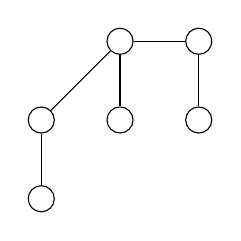
\begin{tikzpicture}[main/.style = {draw, circle}]
    \node[main] (A) {};
    \node[main] (B) [left of=A] {};
    \node[main] (C) [below of=A] {};
    \node[main] (D) [left of=C] {};
    \node[main] (E) [left of=D] {};
    \node[main] (F) [below of=E] {};

    \draw (A) -- (B);
    \draw (A) -- (C);
    \draw (B) -- (D);
    \draw (B) -- (E);
    \draw (F) -- (E);
\end{tikzpicture}
  \caption{An example of a graph.}
  \label{figGraphExample}
\end{figure}
\end{center}

\cite[Chapter 1]{sourceDiestel}
\cite[Chapter 1]{sourceGWA}
\cite[Section 9.1]{sourceArmen}

% Does this add anything?

\section{Hyper Graphs}
A hyper graph is similar to a normal graph.
But in a hyper graph edges connect multiple nodes, usually more than 2.
A hyper edge \DIFdelbegin \DIFdel{which }\DIFdelend \DIFaddbegin \DIFadd{that }\DIFaddend is 2-regular is a "normal" graph.
The "normal" graph can be seen as a special case of the hyper graph.

Another way of phrasing it is that an edge is a set of nodes instead of a pair.

A hyper graph is the kind of graph the no rainbow problem is interesting for.

\begin{center}
\begin{figure}[h]
\centering
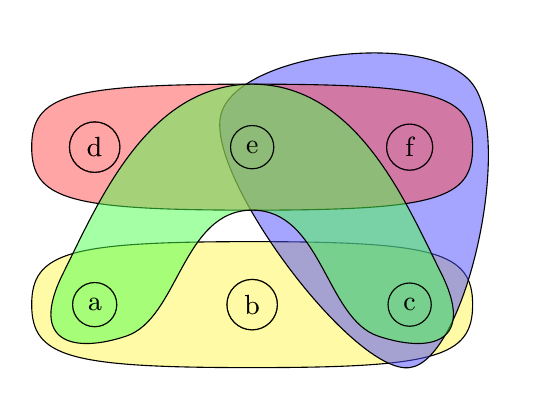
\begin{tikzpicture}[main/.style = {draw, circle}]
    \node[main] (a) at (0,2) {a};
    \node[main] (b) at (2,2) {b};
    \node[main] (c) at (4,2) {c};
    \node[main] (d) at (0,4) {d};
    \node[main] (e) at (2,4) {e};
    \node[main] (f) at (4,4) {f};

    \begin{scope}[fill opacity=0.5]
    \filldraw[fill=yellow!70] 
        plot [smooth cycle, tension=1.5]
        coordinates {
          ($(a)+(-0.8,0)$) 
          ($(b)+(0,0.8)$) 
          ($(c)+(0.8,0)$)
          ($(b)+(0,-0.8)$) 
        };

    \filldraw[fill=blue!70] 
        plot [smooth cycle, tension=0.8]
        coordinates {
          ($(c)+(0,-0.8)$) 
          ($(f)+(0.8,0.8)$) 
          ($(e)+(-0.4,0.4)$)
        };

    \filldraw[fill=red!70] 
        plot [smooth cycle, tension=1.5]
        coordinates {
          ($(d)+(-0.8,0)$) 
          ($(e)+(0,0.8)$) 
          ($(f)+(0.8,0)$)
          ($(e)+(0,-0.8)$) 
        };

    \filldraw[fill=green!70] 
        plot [smooth cycle, tension=1.0]
        coordinates {
          ($(c)+(-0.4,-0.4)$) 
          ($(c)+(0.4,0.4)$) 
          ($(e)+(0,0.8)$)
          ($(a)+(-0.4,0.4)$) 
          ($(a)+(0.4,-0.4)$) 
          ($(e)+(0,-0.8)$)
        };

    \end{scope};

    \node[main] (a) at (0,2) {a};
    \node[main] (b) at (2,2) {b};
    \node[main] (c) at (4,2) {c};
    \node[main] (d) at (0,4) {d};
    \node[main] (e) at (2,4) {e};
    \node[main] (f) at (4,4) {f};
\end{tikzpicture}
  \caption{An example of a hyper graph.}
  \label{figHyperGraphExample}
\end{figure}
\end{center}

% Show the other way of rendering them

The hyper graph shown in figure \ref{figHyperGraphExample} is $3$-regular.
A hyper graph is $r$-regular if and only if all edges connect $r$-different nodes.
\cite{sourceHyper}

\subsection{Node coloring as related by the no rainbow problem}
A node coloring is a mapping from nodes to colors.
There are usually constraints on what colors can be part of an edge.
The color of a node is denoted as $c(a)$, where $a$ is the node and $c$ is the coloring.
Since a coloring is a mapping it can be thought of as a function that takes you from a node to the color of the node.
A color is usually a letter or a number.

The constraints added in the no rainbow problem are
\begin{enumerate}
  \item No edge can have all r-colors -- no rainbow edges
  \item All colors have to be represented in the graph -- the coloring is surjective
\end{enumerate}

An example of a valid coloring in the no rainbow problem for the graph presented above is $c(d)=0, c(b)=1, c(*)=2$, where $*$ denotes all other nodes.
There are a lot more valid colorings, though this coloring is particularly simple.
The validity of a coloring is dictated by the edges added in the graph.
A hyper-graph with the maximum number of edges (called a complete graph) has no valid no-rainbow coloring.
A hyper-graph without any edges is trivial to find a no-rainbow coloring for.
The cases in between are the main topic of this thesis.

\cite{sourceHyper}
%DIF <  Is a complete r-regular subgraph enough to disprove there is a no-rainbow coloring? 
%DIF >  Is a complete r-regular subgraph enough to disprove there is a no-rainbow coloring? Yes.

\section{\DIFdelbegin \DIFdel{The existing algorithms}\DIFdelend \DIFaddbegin \DIFadd{Asymptotic Computational Complexity}\DIFaddend }
\DIFdelbegin \DIFdel{TBA
}\DIFdelend \DIFaddbegin \DIFadd{Sometimes called asymptotic time complexity is a theoretical basis for evaluating algorithms.
The asymptotic computational complexity of an algorithm shows how the run time
of the implemented algorithm scales given infinitely large inputs.
}\DIFaddend 

\DIFdelbegin \section{\DIFdel{Algorithm basics}}
%DIFAUXCMD
\addtocounter{section}{-1}%DIFAUXCMD
\DIFdel{TBA
}\DIFdelend \DIFaddbegin \DIFadd{There are multiple kinds of asymptotic computational complexity. The most used
one -- and the one presented in this paper -- is the "big-O" notation. "Big-O"
gives the highest upper bound of this theoretical runtime -- or the worst-case
computational complexity. Examples usually make things clearer, so let us look at an algorithm.
One intuition for the computational complexity is to "count the number of steps".
}\DIFaddend 

\DIFaddbegin \begin{algorithm}
\caption{\DIFadd{A slow exponentiation algorithm}}\label{algDivSlow}
\KwData{$a,b \in \mathds{Z}, \quad b \le 0$}
\KwResult{$a^b$}
\DontPrintSemicolon
\SetKwFunction{FExp}{Exp}
\SetKwProg{Fn}{Function}{:}{end}

\Fn{\FExp{$a$, $b$}}{
  $x \gets 1$ (Runs 1 time.)\;
  \While(\lparen Runs $b$ times, with $K$ steps.\rparen){$b \le 0$}{
    $x \gets x * a$\; 
    $b \gets b - 1$\;
  }
  \KwRet $x$ (Runs 1 time.)\;
}
\end{algorithm}

\DIFadd{We assume multiplication can be done in constant time -- it always takes at most $K$ units of time to do a multiplication.
The algorithm \ref{algDivSlow} will perform $ 2 + Kb $ steps, where $K$ is some
constant. We can rewrite this using "Big-O" notation as $O(1 + Kb)$. The expression can be
simplified to remove constants that become insignificant if the
input is sufficiently large. Then we get $O(2 + Kb) = O(b)$, since both $1$ and $K$ are constants. 
Normally the asymptotic time complexity is defined based on the size of the input not the magnitude of the value.
The size of the input is measured in number of bits called $n$. When we add a bit to $b$ we multiply the steps by 2,
thus $O(b) = O(2^n)$.
}

\DIFadd{There are other ways to reason to this conclusion.
One other way is to realize we have to visit all numbers between $0$ and $b$.
In binary this means visiting all possible combinations of 0s and 1s that are needed to describe $b$.
We have 2 choices for $n$ bits. All combinations have to be visited. So we visit $O(2^n)$ numbers in the worst case.
\mbox{%DIFAUXCMD
\cite[Chapter 3]{sourceAlgoBook}
}\hskip0pt%DIFAUXCMD
}

\DIFadd{A common error is to claim algorithm \ref{algDivSlow} runs in $O(n)$ -- linear time. This is incorrect.
}

\DIFadd{Aside from $O$ there is also $O*$. $O*(x^n)$ allows us to discard polynomial factors as well. For example $O*(x^n)$ would allow the algorithm to run in $O(2^nx^n)$.
}

\section{\DIFadd{Constraint Satisfaction Problems}}
\DIFadd{Constraint satisfaction problems -- often called CSPs -- is a kind of mathematical problem where a finite set of constraints should be fulfilled. Let us consider some examples of these problems.
}

\DIFadd{One very relevant kind of constraint satisfaction problem is node coloring of hyper graphs.
Constraints are put on what colors can be put where. In the no rainbow problem all colors should never be part of an edge, but all colors should be present in the graph. What makes this problem tricky is that changes locally (to the nodes in an edge) can affect other parts of the graph -- since a node can be part of multiple edges.
}

\DIFadd{Another well known constraint satisfaction problem is SAT -- which is further discussed in section \ref{secSAT}.
}

\section{\DIFadd{SAT, k-SAT and 3SAT}}
\DIFadd{SAT is a very central problem in theoretical computer science. 3SAT is the
hinge pin on which P versus NP rests -- an efficient algorithm for solving 3SAT
solves P versus NP.
}

\DIFadd{SAT, k-SAT and 3SAT ask if logical formulas are satisfiable (there is an assignment in which the expression is true).
The difference between the 3 problems is the input. SAT takes any formula in
CNF-format (conjunctive normal form) -- all clauses are separated by "and"s and
in clauses only negation, variables and "or" is allowed.
}

$$
  \DIFadd{(\tikzmark{v1}a\tikzmark{v2} \vee b \vee c) \tikzmark{w1}\wedge\tikzmark{w2} (\overline{c} \vee d \tikzmark{o1}\vee\tikzmark{o2} e) \wedge \tikzmark{c1}(a \vee \overline{c} \vee e)\tikzmark{c2}
}$$
\begin{figure}[h]

\begin{tikzpicture}[overlay, remember picture, main/.style = {}]

  \node[main, color=blue] (var) at (4,0.3) {variable};
  \node[main, color=green] (conj) at (6,0.3) {conjunction};
  \node[main, color=red] (clause) at (10,0.3) {clause};
  \node[main, color=cyan] (dis) at (8.3,0.3) {disjunction};

  \draw[-, line width=3mm, opacity=0.5, color=blue] ([yshift=1mm]pic cs:v1) -- ([yshift=1mm]pic cs:v2);
  \draw[-, line width=3mm, opacity=0.5, color=green] ([yshift=1mm]pic cs:w1) -- ([yshift=1mm]pic cs:w2);
  \draw[-, line width=3mm, opacity=0.5, color=red] ([yshift=1mm]pic cs:c1) -- ([yshift=1mm]pic cs:c2);
  \draw[-, line width=3mm, opacity=0.5, color=cyan] ([yshift=1mm]pic cs:o1) -- ([yshift=1mm]pic cs:o2);

  \draw[color=blue] (var) -- (pic cs:v1);
  \draw[color=green] (conj) -- (pic cs:w1);
  \draw[color=red] (clause) -- (pic cs:c1);
  \draw[color=cyan]  (dis) -- (pic cs:o1);

\end{tikzpicture}
  \caption{\DIFaddFL{A labeling of a logical expression. An example of input to 3SAT.}}
  \label{figExSAT}
\end{figure}


\DIFadd{An example labeling of the  parts of a logical expression is seen in figure
\ref{figExSAT}. 3SAT requires all clauses to have exactly 3 variables. k-SAT requires all clauses to have exactly k variables. SAT puts not constraints on the causes. But the formula has to be in conjunctive normal form (CNF).
}




\chapter{\DIFadd{Related Work}}
\DIFadd{Exhaustively studies of the no rainbow problem have not been done. There are however a plethora of related problems.
These related problems are more broadly studied.
}

\section{\DIFadd{Exact Algorithms for No-Rainbow Coloring and Phylogenetic Decisiveness}}
\DIFadd{"Exact Algorithms for No-Rainbow Coloring and Phylogenetic Decisiveness" are currently the fastest algorithms.
Two algorithms are presented. One deterministic and one non-deterministic. Both
algorithms use the idea of searching similar potential solutions for a fixed
depth, and then trying again. The non-deterministic algorithm samples the
solution space randomly, while the deterministic algorithm samples a specific
structure. The different search patterns are visualized in figure \ref{figNoRainbowSearchPattern}. \mbox{%DIFAUXCMD
\cite{sourceNoRainbow}
}\hskip0pt%DIFAUXCMD
}

\begin{center}
\begin{figure}[h]
\centering
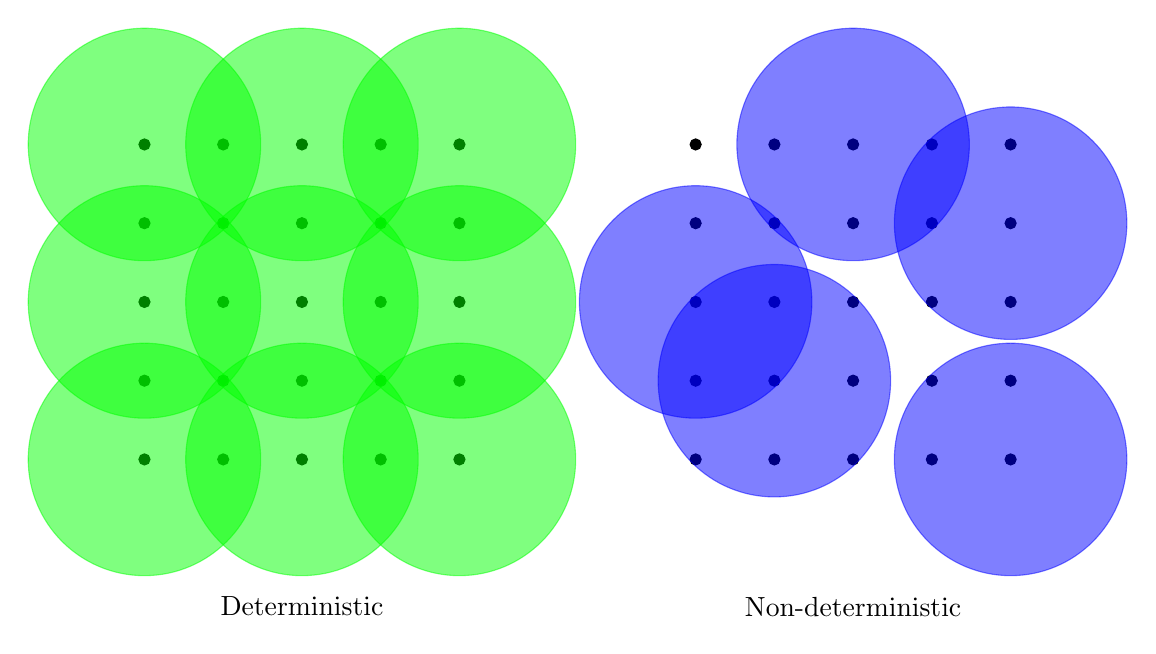
\begin{tikzpicture}
  \newcommand\circleRadius{42pt}

  \foreach \x in {0,...,4}{
    \foreach \y in {0,...,4}{
      \filldraw[black] (\x,\y) circle (2pt);
    }
  }

  \foreach \x in {0,2,4}{
    \foreach \y in {0,2,4}{
      \filldraw[green, opacity=0.5] (\x,\y) circle (\circleRadius);
    }
  }
  \draw (2,-1.5) node[label=below:Deterministic]{};

  % SHIFTED +(4+3,0)
  \foreach \x in {7,...,11}{
    \foreach \y in {0,...,4}{
      \filldraw[black] (\x,\y) circle (2pt);
    }
  }

  \filldraw[blue, opacity=0.5] (8,1) circle (\circleRadius);
  \filldraw[blue, opacity=0.5] (7,2) circle (\circleRadius);
  \filldraw[blue, opacity=0.5] (11,0) circle (\circleRadius);
  \filldraw[blue, opacity=0.5] (9,4) circle (\circleRadius);
  \filldraw[blue, opacity=0.5] (11,3) circle (\circleRadius);
  \draw (9,-1.5) node[label=below:Non-deterministic]{};


\end{tikzpicture}
  \caption{\DIFaddFL{A visualization of how the deterministic and non-deterministic algorithms tries different colorings. Each black dot is a potential solution. The colored circles show the searched adjacent solutions.}}
  \label{figNoRainbowSearchPattern}
\end{figure}
\end{center}

\section{\DIFadd{A Probabilistic Algorithm for k-SAT and Constraint Satisfaction Problems}}
\citeauthor{sourceProbAlgo} \DIFadd{proposes a very simple algorithm for solving k-SAT.
The algorithm is then generalized to all constraint satisfaction problems. The
algorithm is faster than most of the known algorithms of the time (1999) and is
similar to the algorithm proposed by }\citeauthor{sourceNoRainbow} \DIFadd{\mbox{%DIFAUXCMD
\cite{sourceNoRainbow}}\hskip0pt%DIFAUXCMD
.
}

\DIFadd{The k-SAT algorithm starts with a random initial guess. The guess is then edited by flipping one assignment of a variable that is part of a clause which is not satisfied. The flipping is repeated until a fixed depth or a solution is found.
How k-SAT searches is visualized in figure \ref{figKSATSearch}.
}

\DIFadd{\mbox{%DIFAUXCMD
\cite{sourceProbAlgo}
}\hskip0pt%DIFAUXCMD
}

\begin{center}
\begin{figure}[h]
\centering
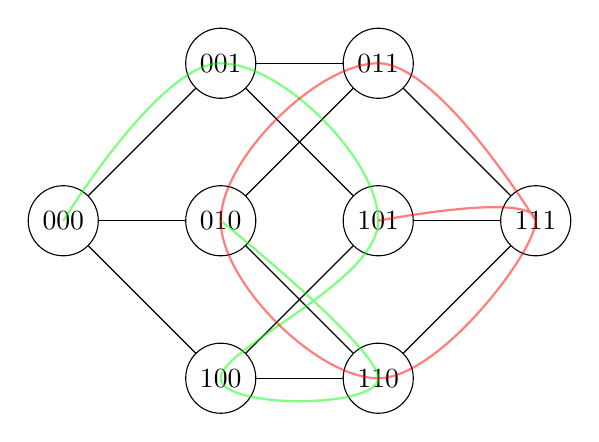
\begin{tikzpicture}[node/.style = {draw, circle}, scale=2]
  \node[node] (a000) at (0,0) {000};

  \node[node] (a001) at (1,1) {001};
  \node[node] (a010) at (1,0) {010};
  \node[node] (a100) at (1,-1) {100};

  \node[node] (a011) at (2,1) {011};
  \node[node] (a101) at (2,0) {101};
  \node[node] (a110) at (2,-1) {110};

  \node[node] (a111) at (3,0) {111};

  \draw (a000) -- (a001);
  \draw (a000) -- (a010);
  \draw (a000) -- (a100);

  \draw (a011) -- (a001);
  \draw (a101) -- (a001);

  \draw (a110) -- (a010);
  \draw (a011) -- (a010);

  \draw (a110) -- (a100);
  \draw (a101) -- (a100);

  \draw (a011) -- (a111);
  \draw (a101) -- (a111);
  \draw (a110) -- (a111);

  \draw[opacity=0.5, thick, smooth, tension=0.7, green] plot[line width=5mm] coordinates { (a000) (a001) (a101) (a100) (a110) (a010) };
  \draw[opacity=0.5, thick, smooth, tension=0.7, red  ] plot[line width=5mm] coordinates { (a101) (a111) (a110) (a010) (a011) (a111) };

\end{tikzpicture}
\caption{\DIFaddFL{A visualization of how the k-SAT algorithm would search for solutions when there are 3 variables. Each node is a potential variable assignment. The lines show how the assignments are searched. The red line is one search and the green line is another search.}}
\label{figKSATSearch}
\end{figure}
\end{center}

\section{\DIFadd{Survey Propagation: an Algorithm for Satisfiability}}
\citeauthor{sourceSurveyProp} \DIFadd{suggest an algorithm which generalizes knowledge about parts of solutions of a SAT-problem. 
When the authors looked at the solution space, they noticed solvers often got stuck in local optimums.
These local optimums forced some variable assignments and created a form of cluster.
By surveying these clusters and generalizing the assignments better guesses can be made.
This algorithm performs incredibly well \mbox{%DIFAUXCMD
\cite{sourceSolutionSpace}}\hskip0pt%DIFAUXCMD
. \mbox{%DIFAUXCMD
\cite{sourceSurveyProp}
}\hskip0pt%DIFAUXCMD
}

\DIFaddend \printbibliography
\DIFaddbegin 

\appendix
\chapter{\DIFadd{Changes after feedback seminar (2022-11-25)}}
\DIFadd{Removed 2 research questions. Added motivation. Added aim. Added delimitations. Fixed typos of multi graph and hyper graph. Corrected typo in title. Moved background to its own chapter. Took feedback from Don and replaced "which" with "that".
}\DIFaddend 

\end{document}
